Este capítulo apresentará trabalhos existentes na literatura que compartilham de objetivos semelhantes ou são comparáveis de alguma forma e contribuem para o desenvolvimento deste trabalho. Os trabalhos descritos nas seções a seguir propõem métodos relacionados a previsão de movimentos para próteses ativas.

% ===================================================================================
\section{Translational Motion Tracking of Leg Joints for Enhanced Prediction of Walking Tasks}
\label{sec:rel_stolyarov}
% ===================================================================================

Neste artigo, \citeonline{stolyarov:2017} propuseram um método de prever tarefas de caminhada utilizando apenas uma IMU (unidade de medição inercial) em uma prótese comercial de uma articulação (tornozelo-pé). Foram classificadas cinco tarefas diferentes: caminhada em solo plano, subida de rampa, descida de rampa, subida de degrau e descida de degrau. Usando apenas a IMU, foi possível ter uma classificação até mais precisa que próteses que usam sEMG, pois, segundo os autores \citeonline{stolyarov:2017}, estas costumam ter ótimos resultados apenas em ambientes de laboratório, mas fora dele dependem de muitos fatores não controlados. A alta acurácia do classificador apresentado sugere que o método tenha ótimos resultados mesmo fora de laboratório.

Algumas limitações deste método são a falta de filtros para tratar problemas comuns do tipo de sensor utilizado, como \textit{drifting}, e a baixa precisão que o algoritmo tem em superfícies escorregadias ou macias.
% 
O estudo do artigo de \citeonline{stolyarov:2017} proporciona ao trabalho aqui proposto a noção de que o uso de acelerômetros e giroscópios pode ser o suficiente para o objetivo proposto, principalmente quando se trata de próteses de baixo custo.

% ===================================================================================
\section{Turn Intent Detection for Control of a Lower Limb Prosthesis}
\label{sec:rel_pew}
% ===================================================================================

No trabalho de \citeonline{pew:2017} foi proposto fazer uma prótese para membros inferiores que tivesse rigidez adaptável em tempo real durante movimentos de virada, prevendo as ações de caminhada e de virada usando técnicas de aprendizagem de máquina, tais como, SVM e KNN. 

A leitura dos dados foi feita a partir da simulação de uma IMU usando captura de movimentos ótica, e o controle da rigidez da articulação foi feita usando um componente chamado VSTA (\textit{variable stiffness torsion adapter}), que podia ser ativado com uma célula de carga comercialmente conhecida como iPecs, como pode ser visto na figura~\ref{fig:rel_turnintent_1}.

\begin{figure}[ht]
	\caption{\label{fig:rel_turnintent_1}Prótese incluindo o VSTA, a célula de carga iPecs e a posição da IMU simulada.}
	\begin{center}
	    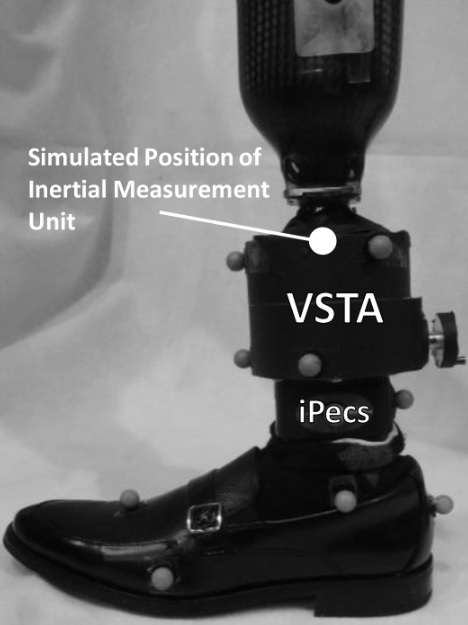
\includegraphics[width=.4\textwidth]{resources/rel_pew_turnintent_1}
	\end{center}
	\legend{Fonte: \citeonline{pew:2017}}
\end{figure}

Para a previsão de ações, foi feita uma comparação entre técnicas de classificação em aprendizagem de máquina: \textit{Bagged Decision Tree Ensemble}, SVM e KNN. Na previsão de caminhada, o SVM teve $85$\% de acurácia, o KNN teve $82$\%, e o Ensemble, $97$\%\todo{Apresentar referências para técnicas listadas}. Na previsão de virada, o SVM teve $96$\%, o KNN, $93$\% e o Ensemble teve $91$\% de acurácia. Embora tenha sido inferior na classificação da intenção de virada, a alta acurácia do \textit{Bagged Decision Tree Ensemble} na detecção de caminhada compensa, o que o torna o algoritmo mais preciso dentre os testados. Também foi constatado, através da IMU simulada, que a acurácia do giroscópio ($83$\% a $90$\%) foi superior à do acelerômetro ($66$\% a $77$\%), o que conclui que o uso apenas do giroscópio pode ser suficiente.

A comparação dos algoritmos feita pelos autores \citeonline{pew:2017} e os testes feitos com a IMU simulada podem ser úteis para este trabalho, pois valida a utilização dos sensores como forma de leitura de movimentos para previsão de intenções.


% ===================================================================================
\section{Automated detection of gait initiation and termination using wearable sensors}
\label{sec:rel_novak}
% ===================================================================================

\citeonline{novak:2013Automated} desenvolveram um método de previsão de início e término de caminhada, a partir de IMUs e uma sola sensível a pressão. O treino foi feito com pessoas com membros intactos e sem deficiências motoras, apenas para desenvolver a técnica. Foram utilizados $12$ sinais das IMUs, passando por filtros de Kalman \cite{kalman:1960}, e $4$ sinais das duas solas. Além disso, os sinais foram classificados utilizando uma árvore de classificação, tanto para detectar os passos individuais quanto para prever as intenções de início e término da caminhada.

No trabalho de \citeonline{novak:2013Automated} foi constatado que é possível detectar o início da caminhada usando a velocidade angular do quadril e ângulo do joelho; e o término utilizando a duração dos passos, e o padrão da pisada na sola para detectar se o passo atual será o último.

Ainda segundo \citeonline{novak:2013Automated}, IMUs são mais eficientes para detectar o término da caminhada, e os sensores nas solas são melhores para detectar os passos individuais. O sistema pode ser adaptado para ser usado em dispositivos como próteses ou exoesqueletos, embora precise ser reduzido para isso, devido à grande quantidade de sensores.

% A técnica apresentada pareceu ser eficiente, porém a grande quantidade de sensores não a torna muito prática fora de um laboratório.

% ===================================================================================
\section{A Novel Design of a Full Length Prosthetic Robotic Arm for the Disabled}
\label{sec:rel_kumar}
% ===================================================================================

% \todo[inline]{\textbf{ATENÇÃO:} Achei esse artigo muito ``engenharia'', pois não fala sobre a classificação em si, e foca muito na construção do braço, incluindo a escolha de materiais.}

O trabalho de \citeonline{kumar:2017} propõe um protótipo de braço prostético robótico (ver Figura~\ref{fig:rel_kumar_1}) controlado por um microcontrolador, com uso de aprendizagem de máquina. Além disso, o objetivo era fazer com que a prótese tivesse movimentos com aspecto humano e o menor torque necessário possível.

\begin{figure}[!htp]
	\caption{\label{fig:rel_kumar_1}Modelagem do protótipo desenvolvida no Solid Works}
	\begin{center}
	    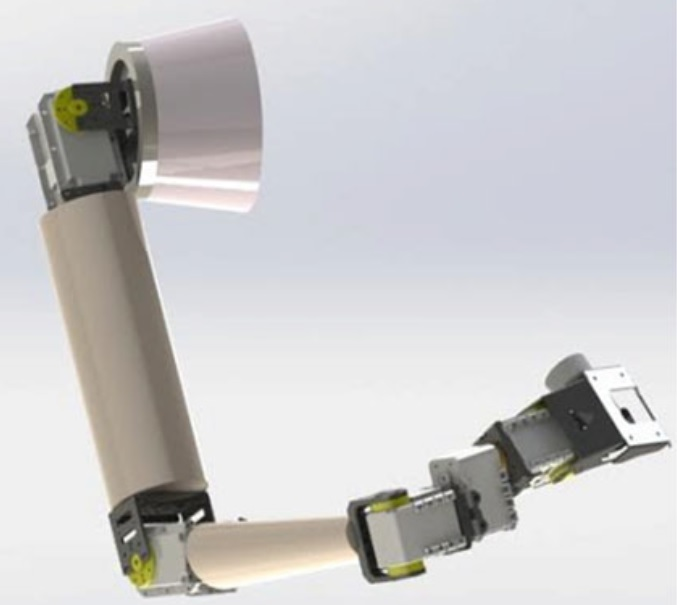
\includegraphics[width=.3\textwidth]{resources/rel_kumar_1}
	\end{center}
	\legend{Fonte: \citeonline{kumar:2017}}
\end{figure}

O protótipo de \citeonline{kumar:2017} foi desenvolvido usando o \textit{software} Solid Works\footnote{<https://www.solidworks.com/>}, e a simulação foi feita com Simulink\footnote{<https://www.mathworks.com/products/simulink.html>} e SimMechanics\footnote{<https://www.mathworks.com/products/simmechanics.html>}. A classificação por aprendizado de máquina foi feita utilizando ANFIS \cite{jang:1993anfis}, um tipo de rede neural artificial, a partir dos dados das simulações\todo{Descrever os resultados da classificação}. Para atuar nos movimentos do braço robótico, foram usados vários servomotores e um microcontrolador PIC16F886.


% ===================================================================================
\section{SmartLeg: An intelligent active robotic prosthesis for lower-limb amputees}
\label{sec:rel_smartleg}
% ===================================================================================

O trabalho de \citeonline{dedic:2011} propõe uma forma de transformar uma prótese passiva disponível comercialmente em ativa, para que seja possível a subida e descida de escadas e outros movimentos que exigem um maior esforço motor. Assim, fez-se necessário o uso de uma fonte de energia externa, que foi feita usando atuadores hidráulicos nas articulações, como visto na Figura~\ref{fig:rel_smartleg_1}.

\citeonline{dedic:2011} também discute o uso de aprendizagem de máquina para garantir conforto aos usuários, pois pode-se adaptar os atuadores para funcionarem melhor com os padrões de andadura do indivíduo, mas isso não foi implementado. Outra ideia mencionada foi o uso de sensores de proximidade e sonares para detecção de obstáculos, algo que também não foi testado, apenas sugerido para o futuro.

\begin{figure}[ht]
	\caption{\label{fig:rel_smartleg_1}Protótipo com dois atuadores hidráulicos: nas articulações do joelho e do tornozelo.}
	\begin{center}
	    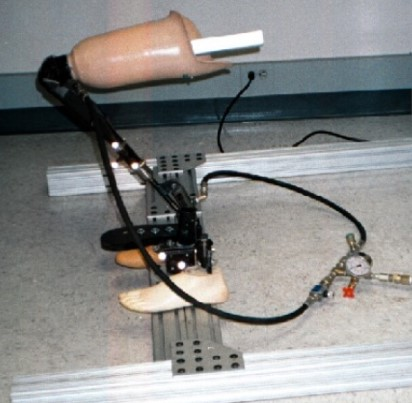
\includegraphics[width=.5\textwidth]{resources/rel_dedic_smart_leg_1}
	\end{center}
	\legend{Fonte: \citeonline{dedic:2011}}
\end{figure}

O protótipo da Figura~\ref{fig:rel_smartleg_1} foi desenvolvido visando baixo custo, pois utiliza uma prótese passiva disponível no mercado, apenas a equipando com atuadores. A coleta de dados realizada permitiu que se comparasse o padrão de caminhada de indivíduos saudáveis com amputados utilizando a prótese, e a prótese produzida permitiu dois graus de liberdade (DOF) com o controle feito por microcontrolador. O maior empecilho é o sistema hidráulico utilizado, que ocupa muito espaço, tornando a versão proposta atual inviável para uso diário.

%\section{Evaluation of shoulder complex motion-based input strategies for endpoint prosthetic-limb control using dual-task paradigm}
%\todo[inline]{\cite{losier:2011}}

%\section{Movement error rate for evaluation of machine learning methods for sEMG-based hand movement classification}
%\todo[inline]{\cite{gijsberts:2014}}
